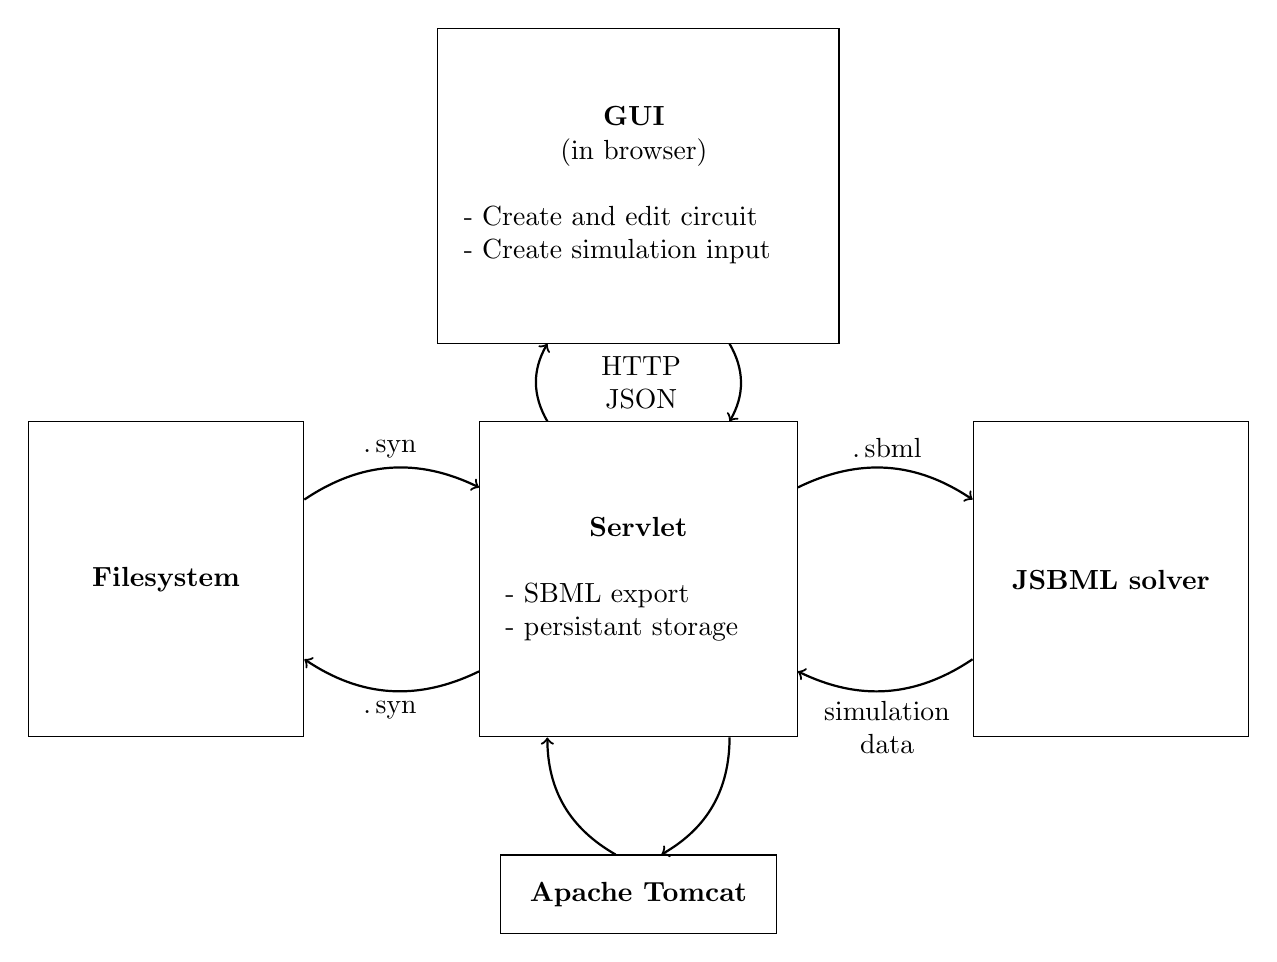
\begin{tikzpicture}
	\tikzstyle{part}=[rectangle, minimum height=4cm, minimum width=3.5cm,draw=black]
	\node[part] (server) at(0,0) {
		\begin{tabular}{ll}
			\multicolumn{2}{c}{\textbf{Servlet}} \\
			\\
			- SBML export & \\
			- persistant storage & \\
		\end{tabular}
	};
	
	\node[part, align=center] (client) at( 0, 5) {
		\begin{tabular}{ll}
			\multicolumn{2}{c}{\textbf{GUI}} \\
			\multicolumn{2}{c}{(in browser)} \\
			\\
			- Create and edit circuit & \\
			- Create simulation input \\
		\end{tabular}
	};
	\node[part, align=center, minimum height=1cm] (tomcat) at (0, -4) {\textbf{Apache Tomcat}};
		
	\node[part] (jsbml) at(6,0) {\textbf{JSBML solver}};

	\node[part] (filesystem) at(-6, 0) {\textbf{Filesystem}};

	
	
	\path[->, thick, bend left]
		(server) edge node[right=.7cm,align=center] {HTTP \\JSON} (client)
		(client) edge (server)
		(jsbml) edge node[below, align=center] {simulation\\ data} (server)
		(server) edge node[above] {.\,sbml} (jsbml)
		(filesystem) edge node[above]{.\,syn} (server)
		(server) edge node[below]{.\,syn}  (filesystem)
		(server) edge (tomcat)
		(tomcat) edge (server);
	
\end{tikzpicture}
